\chapter{Developer Documentation} % Developer guide
\label{ch:impl}

\section{Specification}
\subsection{The problem}
The core problem is rather simple: there are no tools available to simulate network bottlenecks, faults, or anything of the sort. Though some tools do implement a set of predefined rules that can be applied\footnote{For example, Cilium has a bandwidth manager that used EDT to limit the bandwidth of egress packets. https://docs.cilium.io/en/v1.9/gettingstarted/bandwidth-manager/}, these are usually very limited.

More elaborate limit rules can be applied and more tools are available if we drop the constraint of being Kubernetes-specific. On machine level, a whole lot of options are available, including CLI tools, daemon services, etc, but these do have disadvantages over Kubernetes-related, EBPF solutions.
\begin{itemize}
	\item Slower: EBPF enables very fast packet handling because it doesn't require packets to be moved into user space. Most tools today don't use EBPF due to it's newness. 
	\item Machine- or application level limits only: Kubernetes constructs such as Pods or Services can't be referenced
	\item Hard to modify: these tools are often old and when they don't suit the usage, the necessary modification is costly - if at all possible. \newline
\end{itemize}

These disadvantages warrant a solution that is both fast and versatile - it needs to have sane defaults while also providing extensibility.

\subsection{Architecture}
\begin{figure}[H]
	\centering
	
\includegraphics[width=\textwidth]{images/archi.png}
	\caption{Application architecture}
	\label{fig:app-arch-impl}
\end{figure}
\noindent
The proposed solution consists of three main parts.
\begin{enumerate}
	\item The Kubernetes cluster: in most cases, this is a preexisting system, unless specifically set up for testing the application
	\item The application: continuously monitors the state of the Kubernetes cluster and applies limits based on it's configuration
	\item The EBPF Virtual Machine: loads the EBPF programs, verifies their code and runs them whenever a packet arrives on the target ingress / egress interface.
\end{enumerate}

These main parts and technologies, with the addition of some glue, play together to form a versatile yet extensible ecosystem and solve the proposed problem.

TODO folytatni

\newpage
\section{Underlying technologies}
\subsection{Kubernetes}
Kubernetes, or K8S for short, is an open source container orchestration system that is simply too vast to properly explain in a BSc thesis. It supports automatic deployment and scaling of containerized workloads and services. It also works as a base for an ecosystem that's built around it. The project was open-sourced by Google\cite{google} in 2014 and gained prominence in the last few years. Today, it's a mature platform to depend on - no matter what kind of service one's running. Chances are, if scale is a concern, Kubernetes is the answer.

\subsubsection{Why use Kubernetes?}
Today, users of online services are used to a high standard - fast response times, no downtime, no data loss, easy usage. This standard requires modern solutions; a single machine in one's garage running a LAMP\cite{lamp} (Linux, Apache, MySQL, PHP) stack won't cut it anymore. In fact, oftentimes a garage full of server equipment won't cut it.

Scaling this big is hard, though, and This is what Kubernetes is trying to mitigate. Using containers, software becomes more manageable. Containers provide an unified system services can run on, without having to care about what kind of system they run on. These can then be started on-demand, for example when there's a load spike, or another container dies. This ensures that the available workforce is always present and can endure the load, no matter what size it is.

\noindent
The main benefits of Kubernetes are:
\begin{itemize}
	\item Load balancing: Kubernetes can ensure that no host gets overloaded and the services remain stable
	\item Scalability: Containers can be started and stopped on-demand. The deployments always fit to the load.
	\item Automation: Kubernetes automatically modifies it's state at a given rate to meet the requirements set by the sysadmins.
	\item Self-healing: Dead or non-responding pods are automatically restarted.
\end{itemize}

\subsubsection{Kubernetes architecture}
\begin{figure}[H]
	\centering
	
\includegraphics[width=\textwidth]{images/archi.png}
	\caption{Basic architecture of Kubernetes internals}
	\label{fig:kube-arch}
\end{figure}
A Kubernetes cluster is made up from two primary components: the control plane (also called the master node), and one or more worker nodes. The former contains the logic required to orchestrate the latter.

\subsubsection{Master node}
The master node has a single instance and combines multiple already existing - and proven by time - technologies that make Kubernetes so flexible.

The core of everything is the kube-apiserver. It provides an \underline{\gls{api}} to configure and monitor everything while also communicating with other parts of the cluster, such as etcd\cite{etcd}, the kube-scheduler, and controller manager. Etcd is used as a reliable key-value storage that holds every piece of data related to the cluster. The kube-scheduler is responsible for assigning worker nodes to Pods that need to be started. Finally, the controller-manager changes the state of the cluster to always fit the load best.

The master node can run on any machine in a cluster, but typically it's either on the same machine as the worker nodes (in \underline{\gls{on-premises}} cases), or it's hosted by a cloud provider.

\subsubsection{Worker node}
The worker nodes - their number can vary - are the workhorse of the cluster. They are used to run Pods that run the target applications - be they online services or \underline{\gls{ml}} learning algorithms.

The worker nodes are controlled by a program called kubelet. Kubelet manages the Pods and the \underline{\gls{cri}}, the container runtime, which is generally, but not limited to Docker\cite{docker} or containerd\cite{containerd}.

Another tool called kube-proxy implements the overlay network used by Kubernetes. This is required because the communication between pods should be private; unauthorized access from the outside is unwanted. Similarly, the Pods shouldn't access resources outside the cluster that aren't explicitly configured.

\subsubsection{Concepts}
\textbf{Pods} are the smallest components used in Kubernetes. As the name suggests, they represent a group of containers that are closely related and should be handled together. Pods are fast to start and shut down by design, as they are often rotated for various reasons, examples being scaling up and down, starting new pods to replace dead ones, etc. \\

\textbf{Services} are used as an abstraction over a group of Pods. Since usually there are more than one pods, something has to act as a \underline{\gls{load-balancer}} to distribute the requests between the running pods. They are also used to expose an application to the (inner) network. \\

\textbf{Ingresses} act as a reverse-proxy and provide an unified channel external requests can enter through. Depending on the specific implementation (for example, NGINX\cite{nginx} and Traefik\cite{traefik} are solid ones, this thesis project uses the latter), they provide various features, the most important ones being dns/port based routing to services, load balancing and \underline{\gls{ssl}} termination. \\

These aforementioned, rather simple concepts enable the sysadmins to build complex, yet highly performant clusters that scale well under even the most extreme loads.

\begin{figure}[H]
	\centering
	
\includegraphics[width=\textwidth]{images/archi.png}
	\caption{A simple Kubernetes cluster configured with two microservices}
	\label{fig:kube-cluster}
\end{figure}

In the figure above, an ingress controller is used to let in traffic on the HTTP and HTTPS ports, routing them to two services that abstract the pods - 3 each - running web microservices. This simple example shows how the Kubernetes objects interact and enable operators to build bloat-less systems.

\newpage
\subsection{EBPF}
EBPF\cite{ebpf} emerged from BPF\cite{bpf-original}, which is a complex system that leverages a virtual machine with a limited instruction set to run user-made programs in the kernel space. This avoids the need to copy each network packet to the user space, granting significant speed gains. These BPF programs interact directly with raw network sockets. \\

Before loading the programs into the kernel, BPF analyzes the source files to make sure they contain only permitted instructions. The instructions in these files are then run sequentally. The execution of the programs is event-driven; they can be attached to various events, such as the arrival or transmission of a network packet.
 
\subsubsection{BPF VM}
BPF uses a virtual machine that runs code made up from a set of instructions conforming to the following format.
\begin{verbatim}
struct sock_filter {
	__u16	code; // Opcode
	__u8	jt;	   // Jump if true
	__u8	jf;    // Jump if false
	__u32	k;    // Instruction-dependent field
};
\end{verbatim}

These instructions are represented as an array of 4-\underline{\gls{tuple}} and are run in a sequence.

\begin{verbatim}
struct sock_fprog {
	unsigned short len; // Number of instructions
	struct sock_filter __user *filter;
};
\end{verbatim}

The BPF virtual machine has a rather simple architecture. A 32 bit wide register - called A - is used as an accumulator and another one - called X - is used as a helper register. The VM also has a 32 bit wide "scratch memory store" - called M - that can store up to 16 values.

BPF has a simple \underline{\gls{risc}} (Reduced Instruction Set Computing) instruction set consisting of load, save, jump, arithmetic and logic operations. A program of these instructions is usually denoted as an array of 4-tuples. \\
 
Full list of instructions:
\begin{center}
 \begin{tabular}{||c c c||} 
 \hline
 Instruction & Addressing mode & Description \\ [0.5ex] 
 \hline\hline
  ld & 1, 2, 3, 4, 12 & Load word into A \\
  \hline
  ldi &  4 & Load word into A \\
  \hline
  ldh &  1, 2 & Load half-word into A \\
  \hline
  ldb & 1, 2 & Load byte into A \\
  \hline
  ldx & 3, 4, 5, 12 & Load word into X \\
  \hline
  ldxi & 4 & Load word into X \\
  \hline
  ldxb & 5 & Load byte into X \\
  \hline
  \hline
  st & 3 & Store A into M[] \\
  \hline
  stx & 3 & Store X into M[] \\
  \hline
  \hline
  jmp & 6 & Jump to label \\
  \hline
  ja & 6 & Jump to label \\
  \hline
  jeq & 7, 8, 9, 10 & Jump on A == <x> \\
  \hline
  jneq & 9, 10 & Jump on A != <x> \\
  \hline
  jne & 9, 10 & Jump on A != <x> \\
  \hline
  jlt & 9, 10 & Jump on A <  <x> \\
  \hline
  jle & 9, 10 & Jump on A <= <x> \\
  \hline
  jgt & 7, 8, 9, 10 & Jump on A >  <x> \\
  \hline
  jge & 7, 8, 9, 10 & Jump on A >= <x> \\
  \hline
  jset & 7, 8, 9, 10 & Jump on A \&  <x> \\
  \hline
\end{tabular}
\captionof{table}{BPF instructions part 1}
\end{center}

\newpage
\noindent
Continued:
\begin{center}
 \begin{tabular}{||c c c||} 
 \hline
 Instruction & Addressing mode & Description \\ [0.5ex] 
 \hline\hline
  add & 0, 4 & A + <x> \\
  \hline
  sub & 0, 4 & A - <x> \\
  \hline
  mul & 0, 4 & A * <x> \\
  \hline
  div & 0, 4 & A / <x> \\
  \hline
  mod & 0, 4 & A \% <x> \\
  \hline
  neg & & !A \\
  \hline
  and & 0, 4 & A \& <x> \\
  \hline
  or & 0, 4 & A | <x> \\
  \hline
  xor & 0, 4 & A \^ <x> \\
  \hline
  lsh &  0, 4 & A << <x> \\
  \hline
  rsh & 0, 4 & A >> <x> \\
  \hline
  tax & & Copy A into X \\
  \hline
  txa & & Copy X into A \\
  \hline
  \hline
  ret & 4, 11 & Return \\
  \hline
\end{tabular}
\captionof{table}{BPF instructions part 2}
\end{center}

\newpage
There are multiple addressing modes each having it's own quirks. The table below explains their behavior.
\begin{center}
 \begin{tabular}{||c c c||} 
 \hline
   Addressing mode & Syntax & Description  \\ [0.5ex] 
 \hline\hline
   0 & x/\%x & Register X \\
   \hline
   1 & [k] & BHW at byte offset k in the packet \\
   \hline
   2 & [x + k] & BHW at the offset X + k in the packet \\
   \hline
   3 & M[k] & Word at offset k in M[] \\
   \hline
   4 & \#k & Literal value stored in k \\
   \hline
   5 & 4*([k]\&0xf) & Lower nibble * 4 at byte offset k in the packet \\
   \hline
   6 & L & Jump label L \\
   \hline
   7 & \#k,Lt,Lf & Jump to Lt if true, otherwise jump to Lf \\
   \hline
   8 & x/\%x,Lt,Lf & Jump to Lt if true, otherwise jump to Lf \\
   \hline
   9 & \#k,Lt & Jump to Lt if predicate is true \\
   \hline
  10 & x/\%x,Lt & Jump to Lt if predicate is true \\
   \hline
  11 & a/\%a & Accumulator A \\
   \hline
  12 & extension & BPF extension \\
   \hline
\end{tabular}
\captionof{table}{Addressing modes of instructions}
\end{center}

\newpage
\subsubsection{EBPF}
\label{sec:ebpfrules}
BPF was originally proposed in 1992, having seen low to moderate success. EBPF, which builds on the original BPF implementation, first appeared in Linux kernel 3.18\cite{kernel-318} released in 2014 and became widely adopted in the last few years. However, it's still somewhat of an underground technology, as it requires more-than-average knowledge about the Linux kernel and it's use cases are quite narrow.

The relative bigger success of EBPF is mainly due to the fact that it not just extended, but reworked the technology from ground up. The VM was expanded to support 64 bit architectures and a variety of things absent form the predecessor.

\subsubsection{EBPF VM}
The re-implemented EBPF VM architecture has eleven general-purpose 64 bit wide registers (r0 - r10) that can also be used in 32 bit mode. R10 is \underline{\gls{read-only}} and contains the \underline{\gls{fp}} It also has a \underline{\gls{pc}} and a 512 byte long \underline{\gls{stack}}.

This new architecture also brought a new instruction format along.
\begin{verbatim}
struct bpf_insn {
	__u8	code;		// Opcode 
	__u8	dst_reg:4;	// Destination register
	__u8	src_reg:4;	// Source register
	__s16	off;		// Signed offset
	__s32	imm;		// Signed immediate constant
};
\end{verbatim}

The new instruction format made it necessary to update the instructions themselves as well. The base stayed the same, but it was extended to support 64 bit wide data and added several new features, for example, function calls and proper branching instructions. The list is too long to include, however it's freely available\cite{ebpf-instructions}.

This new architecture is much more powerful than the limited functionality the original BPF system provided. This introduced the requirement of having a \underline{\gls{verifier}} that scans the code and rejects to load anything outside the allowed parameters. EBPF has three main rules that make it safe to use.
\begin{itemize}
	\item Only forward jumps are allowed. This ultimately means that loops are forbidden, guaranteeing the termination of the program.
	\item All memory accesses are validated. The kernel must not allow the programs to tamper around in the memory.
	\item The program must have no more than 4096 instructions.
\end{itemize}

These basic rules together ensure that all BPF programs run fast and terminate without exceptions.


\subsubsection{EBPF for packet filtering}
Even though BPF's original purpose was - as the name suggests - packet filtering, EBPF broadened the tool's functionality. Nowadays, a hook can be virtually added anywhere on the machine, be it in the kernel or user space code. These can be done using \underline{\gls{kprobe}}s and \underline{\gls{uprobe}}s respectively.

Staying on the topic, packet filtering can be done through attaching EBPF programs to ingress or egress \underline{\gls{socket-buffer}}s. Ingress socket buffers are where transmitted data is passed to a process, and egress socket buffers are where the process outputs data that gets transmitted back onto the network. These socket buffers are located in kernel space and are managed by the Linux \underline{\gls{tc}}. \\

An example of a simple bandwidth limiter EBPF program would be attached to the egress of a process. It would either let packets pass, or throw them away based on their length and the time elapsed since the last packet. More sophisticated solutions would delay the packets and not throw them away. This latter is called \underline{\gls{edt}} filtering.

\newpage
TODO EBPF DATAPATH kep https://docs.cilium.io/en/v1.8/concepts/ebpf/lifeofapacket/
some bs about the datapath

\subsection{Go}
Golang\cite{go} is an open-source programming language that focuses on code simplicity, efficiency and reliability. It has a very opinionated view on how code should look and behave, which is referred to as idiomatic way. Go also has a wide set of concurrency mechanisms which make it perfect for writing networking and multi-core applications. \\

The language was designed at Google\cite{google} by Rob Pike\cite{rpike}, and Ken Thompson\cite{kthompson} themselves, among others, first released in 2012\cite{go-1}.

Under the hood, Go is a \underline{\gls{compiled}} and \underline{\gls{statically-typed}} language that resembles C\cite{c}, but unlike this latter, it has a \underline{\gls{garbage-collector}}, it's \underline{\gls{memory-safe}}, and has an actually usable standard library. \\

The project uses Go as the main language for the application because there were no special requirements, any other general-purpose languages would have worked, for example C++ or Python. Go's preference of simplicity and my familiarity with the language were the main reasons to pick it. \\

One important thing about Go is that it doesn't support most classic \underline{\gls{oop}} paradigms such as inheritance or polymorphism. Instead, Go has an unique take on what OOP should be like. This by the way, often throws off developers getting acquainted with the language as it feels alien at first. For this same reason, the thesis doesn't include any complex OOP features - they would be pointless anyway as the internal structure is kept simple.

\newpage
\subsection{Other Linux technologies}
\subsubsection{Control Group V2}
Another relatively recent technology utilized by the thesis project is cgroup v2\cite{cgroup}. Cgroup is a hierarchical system where groups can contain other groups and every process belongs to exactly one group. These groups are addressable and are used to distribute system resources, for example \underline{\gls{cpu}} capacity or usable \underline{\gls{ram}}. \\

The old V1 version is now deprecated and is superseded by V2. It unifies the then scattered layout of the hierarchy in one \underline{\gls{tree}}. Though it's widely available, some projects still don't fully support it, one example being K3S (a K8S distribution, also used by this project) until very recently.

The thesis project uses the cgroup V2 system to address processes during the EBPF attachment procedure.

\subsubsection{Tools}
\textbf{Bpftool}\cite{bpftool} is a Linux utility that's used to load and unload BPF code as well as to inspect BPF logs and maps. This latter can be done by running the following command.
\begin{verbatim}
$ sudo bpftool p t
\end{verbatim}

\textbf{Clang}\cite{clang}, part of the LLVM project is a C/C++ compiler that is able to compile EBPF bytecode. At the time of writing this thesis, this compiler is the most reliable way to generate EBPF programs.

\newpage
\section{Implementation}
\subsection{The application}
This section will explain the actual implementation of the application and it's subprograms. The application is written in Go because of it's simplicity and robustness. As the main application is just orchestrating other technologies to work together, no complex structure was required.

\begin{figure}[H]
	\centering
	
\includegraphics[width=\textwidth]{images/archi.png}
	\caption{TODO folyamatabra ami mutatja, hogy keresi a serviceket podokat a cucc es tolti be}
	\label{fig:loading-arch}
\end{figure}

The structure of application follows a simple workflow. On startup, the application connects to the Kubernetes API, sweeping the cluster for services and pods that require EBPF programs to get hooked on. It also starts to watch events happening in the cluster, in case pods get replaced.

When finding a service that is configured to use a limit, the corresponding pods are also searched and the limit is applied on them. When finding a direct pod limit, it's directly applied.

The process of applying EBPF programs that implement limits consists of compiling the EBPF programs with the given parameters, loading them into the kernel, and attaching these programs to the cgroup of the given pod's processes.

\subsubsection{Startup}
In Go programs, the entry point is a main() function in the package main. This is where the program flow starts.

When starting the application, the first thing that happens is locating the kubeconfig file. This file can be either in the home folder of the user, or anywhere else - this location can be passed to the application through a command-line parameter. After locating the kubeconfig file, the contents are interpreted and the application attempts to connect to the Kubernetes API. \\

A struct - the Go equivalent of class - called PodManager is responsible for the business logic. 
\begin{figure}[H]
	\centering
	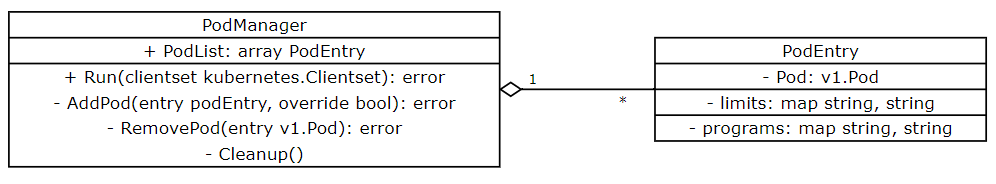
\includegraphics[width=\textwidth]{images/uml.png}
	\caption{Class diagram of the pod manager code section}
	\label{fig:uml}
\end{figure}

The PodManager holds all the data related to the program execution - information about pods and their corresponding limits and EBPF programs - and also contains the core logic. The execution start when the Run() method is called. This method executes the following 3 steps in a strict order:

\begin{enumerate}
	\item Looking for configured services: most often, limits will be applied on this level.
	\item Looking for configured pods and deployments: this must come after looking for services; pod-level limits overwrite service-level ones, providing a hierarchical solution.
	\item Setting up an even watcher for pods through the Kubernetes API: this step comes last because at this point, we only want to find changes in the cluster.
\end{enumerate}

When looking for services and pods, the software is checking their annotation parameter to see if there are any limits present. In the last step, the event watcher is set up and it runs until the application exits. This enables dynamic loading and unloading of EBPF programs whenever the cluster is changed.

\subsubsection{EBPF program loading}
The first step of EBPF program loading is to actually compile the object code. This is done using the Clang compiler. The pre-implemented programs' sources are stored in the bpf folder. Every program is compiled independently to provide custom settings through the macros.

During compilation, the kernel headers are linked to the object code, and specific macros are set depending on which program is being compiled. These macros are used to bypass a limitation of the EBPF VM, namely that it doesn't allow the programs to be parametrized. Although EBPF does support maps that are accessible from user space, these don't fit the use case. \\

After compilation, the next step is to actually load the object-code into the kernel. This is done through a system call, which is done by the bpftool utility automatically invoked though command line. Upon loading the object-code, the EBPF verifier examines the code and makes sure it's safe to run. If the verifier accepts the code, it gets compiled to machine code. The internal compiler also optimizes the code, making it run at speeds similar to natively compiled kernel code. \\

Once the EBPF program is loaded into the kernel, it must be attached to a process. This process is referred to by it's cgroup, which is found in the \texttt{/sys/fs/cgroup/} folder. After the attachment, the system is live and the limits should instantly begin to take effect. This can be made sure using the following command.
\begin{verbatim}
$ sudo bpftool p t
\end{verbatim}

If the process finished successfully, the command should show packet transmission and whether they were dropped or not.

\subsubsection{Cleanup}
On exiting (and pod removal in the cluster), cleanup is done. This includes removing temporary artifacts as well as unloading and deattaching EBPF programs - even though they automatically get cleaned up if the process they are attached to stop. This process is done for the sake of completeness.

These processes happen in reverse order - meaning first the program is deattached from the cgroups, after which they are unloaded, and finally, the artifacts (the object files) are deleted.

\newpage
\subsection{Implemented rules}
Although the thesis project is extensible with custom user-made EBPF programs, it comes with prebuilt ones that cover the most frequently required features. The following sections describe the inner working of these programs.

\subsubsection{Bandwidth limit}
The bandwidth manager's sole purpose is to limit the bandwidth used by a specific Pod's \underline{\gls{ingress}} or \underline{\gls{egress}}. To reach this goal, it employs an algorithm called \underline{\gls{tbf}} which drops packets that are too big compared to the time elapsed since the last one. This is a rather simple solution, keeping the average bandwidth below a specified threshold. \\

The pros of TBF include simplicity and high processing speed. This can be useful in cases where low \underline{\gls{latency}} is an absolute necessity, for example serving multimedia content on the web. The high speed of the algorithm is due to its simplicity; the low latency is guaranteed by the fact that packets are either instantly let-through, or dropped. Below-limit bandwidth is always instantly forwarded. \\

The cons arise from the nature of the algorithm - packets above the bandwidth limit get dropped. This means that only \underline{\gls{tcp}} transmissions are reliable, as they resend packets that weren't acknowledged. \underline{\gls{udp}} doesn't do this, requiring proper user-made \underline{\gls{netcode}} to handle dropped packets. \\

Staying at the topic of \underline{\gls{transport-layer}} protocols, TCP also shapes the speed of the data transmission dynamically. This is helpful because as packets get dropped, TCP throttles the speed, requiring the bandwidth manager to drop less packets. UDP doesn't have any similar features.

\newpage
\textbf{The TBF algorithm} uses a bucket that gets filled with "tokens". Packets take tokens to send, and if a packet would  completely drain the bucket, it gets dropped, otherwise let through. More formally:
\texttt{
\begin{enumerate}
	\item Tokens are added to a bucket with 1/ rate interval.
	\item A bucket can hold at most b tokens.
	\item When a packet arrives (of length p):
	\begin{enumerate}
    	\item If the bucket has more than p tokens, the same amount is removed and the packet is let through.
    	\item Otherwise, the packet is discarded.
    \end{enumerate}
\end{enumerate}
}
EBPF is event-driven - in this case, these events are packet arrivals on either the ingress or the egress interface - therefore this algorithm requires slight modifications to work properly, namely the token addition is the part that requires discrete time steps instead of being continuous. The implemented algorithm is the following.
\texttt{
\begin{enumerate}
	\item When a packet arrives:
	\item Calculate the time between the last packet and the current packet's arrival as dT.
	\item Add dT * rate amount of tokens to the bucket
	\item If the bucket has more than p tokens, the same amount is removed and the packet is let through.
	\item Otherwise, the packet is discarded.
	\item Update the time of the last packet's arrival
\end{enumerate}
}
The algorithms may slightly differ, but in essence, both implement the same idea: only let through packets through where the average bandwidth calculated as packet size * (time of last packet - time of current packet) is below the threshold. This limits the maximal available bandwidth.

There are also other TBF algorithms that extend the basic idea of it, though they aren't implemented in the project as they're not required for the original purpose. Examples include the leaky bucket and the hierarchical token bucket algorithms.

\subsubsection{Packet loss}
Simulating packet loss is useful in cases where network-congestion testing is important. It can be configured for Pods' ingress or egress interfaces. There are two variations provided by the implementation, one using uniform and the other using exponential distribution.

Simulating probability-based things is very difficult without \underline{\gls{float}} or an usable standard library. Unfortunately, neither of those are available in the Linux kernel. To further complicate things, a \underline{\gls{rng}} is also required, not provided by the kernel by default. \\

For random-numbers, both implementations use the BPF helper function funcname TODO provided by TODO. This generates a random 32 bit value which is then used as a base for both distributions. The absence of floating-point numbers is circumvented by only using integer calculations; this does lose precision but for the use case, it's good enough. \\

Using the \textbf{uniform-distribution}, a percentage of packets can be dropped. This comes useful simulating congestion that happens on a regular basis, such as crowded Wi-Fi. This version of the loss manager is pretty straightforward, requiring little explanation. The random 32 bit number is interpreted as an unsigned integer modulo 100, and the output is compared to the given percentage provided in configuration. The packet is then passed through or dropped based on this. \\

The \textbf{exponential-distribution} has a threshold above which it throws packets. Using this distribution, edge-cases can be simulated - as the top-end of the distribution is rather rare.

Exponential distribution can be calculated from uniform one. Given a variable U conforming to uniform-distribution between [0,1), the following formula can be used to calculate the exponential-distributed value:
$$\xi = -\frac{1}{\lambda}\ln(1-U)$$

\newpage
The implementation is somewhat awkward because of the absence of floating point integers and math libraries, this equation can't be used. Instead, since no better tools are available inside the kernel, a lookup table containing a predefined exponential curve is used. This is somewhat of a hack-ish solution, but after careful consideration, it was chosen not only because of the lack of better methods, but also for it's speed. Very few - if any - other solutions beat the speed of lookup tables.

\begin{figure}[H]
	\centering
	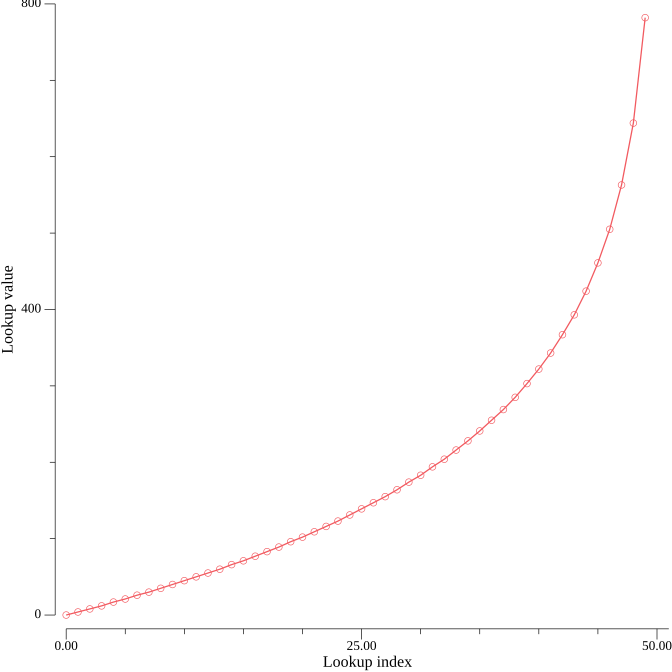
\includegraphics[width=\textwidth]{images/lookuptable.png}
	\caption{Lookup table for exponential distribution}
	\label{fig:exp-lookup-table}
\end{figure}

The lookup table itself is implemented with a switch statement, instead of using an array. This is due to the EBPF verifier, which won't let the program offset an array with a random value - not even in a sanitized and bound-checked way.

The exponential distribution code is straightforward as well. Given the random 32 bit unsigned integer modulo 50 (this number was chosen for keeping the size of the lookup table manageable), the corresponding exponential value can be found. This is then compared to a threshold, and the packet is passed through or dropped based on the comparison.


\subsubsection{EDT}
Another way of bandwidth limiting is the EDT algorithm. Instead of dropping, this algorithm delays packets to ensure the fixed bandwidth threshold is not exceeded. Due to its nature, this algorithm only works for egress interfaces, and it's not fit for our use case.

Nevertheless, it's implemented as it may come useful later in the future. It can be found in the \texttt{bpf/edt.c} file. \\

The algorithm uses a variable called t\_next that is set in the previous packet transmission. This variable is used to determine the earliest point the next packet can leave. The delay of a packet is calculated as packet\_size times bitrate. If the packet is sent after t\_next, it's passed through and t\_next is set to the current time plus the delay.

If the packet is before t\_next, the delay is added to the packet's timestamp and it's passed through - meaning it will be resent at a later date.

\newpage
\section{Testing}
The correctness of the software bundle is ensured with both tests and benchmarks. The tests are performed on the code, while benchmarks are measured on the running systems.

\subsection{Unit tests}
Since the main application is kept simple, meaning it has neither complex structure or user-interface, testing the code base is simple as well, as there are only a few things that can be tested. \\

Due to how Go implements the type system, \underline{\gls{mock}}ing is rather verbose. Polymorphism is achieved through interfaces, which are types having only methods. Actual types can implement these, and therefore the interface itself, and can be passed as such. This means mocking for example the Kubernetes API would mean all of its functions need to be re-implemented, which is simply not feasible. For this reason, dependencies such as the Kubernetes API aren't tested; they should be tested in a stand-alone manner anyway. \\

\noindent
The following basic features are tested:
\begin{itemize}
	\item Compiling programs
	\item Deleting programs
	\item Loading programs
	\item Unloading programs
\end{itemize}

The EBPF programs themselves cant be tested in any way due to their specific format and the fact that tests can not be run in the Linux kernel.

\newpage
\subsection{Benchmarks}


//todo
benchmarks
reloading doesnt work